\documentclass[]{article}
\usepackage{lmodern}
\usepackage{amssymb,amsmath}
\usepackage{ifxetex,ifluatex}
\usepackage{fixltx2e} % provides \textsubscript
\ifnum 0\ifxetex 1\fi\ifluatex 1\fi=0 % if pdftex
  \usepackage[T1]{fontenc}
  \usepackage[utf8]{inputenc}
\else % if luatex or xelatex
  \ifxetex
    \usepackage{mathspec}
    \usepackage{xltxtra,xunicode}
  \else
    \usepackage{fontspec}
  \fi
  \defaultfontfeatures{Mapping=tex-text,Scale=MatchLowercase}
  \newcommand{\euro}{€}
\fi
% use upquote if available, for straight quotes in verbatim environments
\IfFileExists{upquote.sty}{\usepackage{upquote}}{}
% use microtype if available
\IfFileExists{microtype.sty}{%
\usepackage{microtype}
\UseMicrotypeSet[protrusion]{basicmath} % disable protrusion for tt fonts
}{}
\usepackage[margin=1in]{geometry}
\usepackage{color}
\usepackage{fancyvrb}
\newcommand{\VerbBar}{|}
\newcommand{\VERB}{\Verb[commandchars=\\\{\}]}
\DefineVerbatimEnvironment{Highlighting}{Verbatim}{commandchars=\\\{\}}
% Add ',fontsize=\small' for more characters per line
\usepackage{framed}
\definecolor{shadecolor}{RGB}{248,248,248}
\newenvironment{Shaded}{\begin{snugshade}}{\end{snugshade}}
\newcommand{\KeywordTok}[1]{\textcolor[rgb]{0.13,0.29,0.53}{\textbf{{#1}}}}
\newcommand{\DataTypeTok}[1]{\textcolor[rgb]{0.13,0.29,0.53}{{#1}}}
\newcommand{\DecValTok}[1]{\textcolor[rgb]{0.00,0.00,0.81}{{#1}}}
\newcommand{\BaseNTok}[1]{\textcolor[rgb]{0.00,0.00,0.81}{{#1}}}
\newcommand{\FloatTok}[1]{\textcolor[rgb]{0.00,0.00,0.81}{{#1}}}
\newcommand{\CharTok}[1]{\textcolor[rgb]{0.31,0.60,0.02}{{#1}}}
\newcommand{\StringTok}[1]{\textcolor[rgb]{0.31,0.60,0.02}{{#1}}}
\newcommand{\CommentTok}[1]{\textcolor[rgb]{0.56,0.35,0.01}{\textit{{#1}}}}
\newcommand{\OtherTok}[1]{\textcolor[rgb]{0.56,0.35,0.01}{{#1}}}
\newcommand{\AlertTok}[1]{\textcolor[rgb]{0.94,0.16,0.16}{{#1}}}
\newcommand{\FunctionTok}[1]{\textcolor[rgb]{0.00,0.00,0.00}{{#1}}}
\newcommand{\RegionMarkerTok}[1]{{#1}}
\newcommand{\ErrorTok}[1]{\textbf{{#1}}}
\newcommand{\NormalTok}[1]{{#1}}
\usepackage{graphicx}
\makeatletter
\def\maxwidth{\ifdim\Gin@nat@width>\linewidth\linewidth\else\Gin@nat@width\fi}
\def\maxheight{\ifdim\Gin@nat@height>\textheight\textheight\else\Gin@nat@height\fi}
\makeatother
% Scale images if necessary, so that they will not overflow the page
% margins by default, and it is still possible to overwrite the defaults
% using explicit options in \includegraphics[width, height, ...]{}
\setkeys{Gin}{width=\maxwidth,height=\maxheight,keepaspectratio}
\ifxetex
  \usepackage[setpagesize=false, % page size defined by xetex
              unicode=false, % unicode breaks when used with xetex
              xetex]{hyperref}
\else
  \usepackage[unicode=true]{hyperref}
\fi
\hypersetup{breaklinks=true,
            bookmarks=true,
            pdfauthor={},
            pdftitle={},
            colorlinks=true,
            citecolor=blue,
            urlcolor=blue,
            linkcolor=magenta,
            pdfborder={0 0 0}}
\urlstyle{same}  % don't use monospace font for urls
\setlength{\parindent}{0pt}
\setlength{\parskip}{6pt plus 2pt minus 1pt}
\setlength{\emergencystretch}{3em}  % prevent overfull lines
\setcounter{secnumdepth}{0}

%%% Use protect on footnotes to avoid problems with footnotes in titles
\let\rmarkdownfootnote\footnote%
\def\footnote{\protect\rmarkdownfootnote}

%%% Change title format to be more compact
\usepackage{titling}

% Create subtitle command for use in maketitle
\newcommand{\subtitle}[1]{
  \posttitle{
    \begin{center}\large#1\end{center}
    }
}

\setlength{\droptitle}{-2em}
  \title{}
  \pretitle{\vspace{\droptitle}}
  \posttitle{}
  \author{}
  \preauthor{}\postauthor{}
  \date{}
  \predate{}\postdate{}



\begin{document}

\maketitle


\section{FUEL CONSUMPTION: MANUAL VS AUTOMATIC
CARS}\label{fuel-consumption-manual-vs-automatic-cars}

\subsection{EXECUTIVE SUMMARY}\label{executive-summary}

This report aims at investigating the following questions:

\begin{enumerate}
\def\labelenumi{\arabic{enumi}.}
\itemsep1pt\parskip0pt\parsep0pt
\item
  Is an automatic or manual transmission better for MPG (miles per
  gallons)\\
\item
  Quantify the MPG difference between automatic and manual transmissions
\end{enumerate}

The analysis is carried out on the dataset mtcars. Due to the small
number of models and the age of the dataset, the results cannot be
generalised to the current population of cars, but can give an insight
within the set of cars considered.

The sole distinction between manual and automatic cars is a poor
predictor of the fuel consumption and other factors more influential
have to be taken into account in a more precise prediction. The other
reason we need to consider other factors is that in the database, manual
cars tend to be imported models generally lighter and smaller, hence
with lower fuel consumption.

To better answer the question we therefore propose a model to predict
fuel consumption which includes, on top of the a/m distinction, the
weight of the car and the number of cylinders. In this context, there is
not a statistically significant difference in fuel consumption between
manual cars and automatic ones.

\subsection{REPORT}\label{report}

The database contains \textbf{32} car models of which \textbf{19} have
automatic transmission and \textbf{13} have manual. The variable ``am''
is \textbf{0} for automatic transmission and \textbf{1} for manual.

A simple t-test confirm that the two transmissions are not from the same
population as the interval does not contain 0 and the p-value
\textbf{0.0014} is sufficiently low (see \emph{Appendix 2}), therefore
there is a statistcally significant difference in the ``mpg'' of the two
groups. For the sake of this projects we assume ``mpg'' to have a normal
distribution, although it looks a little skewed.

We consider a linear model with ``am'' as a predictor and ``mpg'' as a
response (see \emph{Appendix 3}). The model performs poorly: R-squared
\textbf{0.36} is very low (1 being best fit, 0 being no fit at all) and
this, together with a Residual Standard Error (RSE) of \textbf{4.822},
suggests that the model is not accurate.

We look therefore at other variables that might be confounders. Let's
call primary the variables that refer to specifications of the car of
the engine (``cyl'', ``disp'', ``drat'', ``wt'', ``vs'', ``am'',
``gear'', ``carb'') and secondary the ones that are performance on the
car (``mpg'', ``hp'', ``qsec'') and therefore consequences of the
primary ones. We are interesting in the outcome of a secondary variable
(``mpg'') with primary variables as predictors. Based on a brief
literature review, the variables that can be relevant to our analysis
are weight, the number of cylinders and the displacement. The rear axle
ratio (``drat'') is also mentioned as having an impact on fuel
consumption. The weight and the number of cylinders can tell a lot about
a car because they are related to the size and power of the engine and
therefore the size and the type of car. Displacement (the amount of fuel
burnt per stroke of the engine) gives similar information about the
engine but in this case it is correlated with cylinders (see
\emph{Appendix 4}) and we therefore use interaction rather than
confounding.\\We will proceed at setting up 5 nested models, verifying
the best fit and then drop redundant variables through an ANOVA test.

A look at the ``wt'' plot of \emph{Appendix 1} we can imagine two groups
of cars, one of light and manual cars and the other of heavy and
automatic cars. The plot in \emph{Appendix 5} suggests that there are
indeed two groups with different reaction to the increase to weight.
Rather than automatic/manuals having different ``mpg'' trend based on
the weight, we suggest that there is a quadratic relationship between
``wt'' and ``mpg'', that is the slope changes with the weight (steeper
on the left side of the graph, flatter on the right). This would explain
why mpg in manuals cars, that are on the left of the graph, have a
steeper slope than automatic ones. Let's have \emph{model1} with the
linear predictor ``wt'' and \emph{model2} where we add ``wt''\^{}2.
Indeed model2 better explains the relationship between ``wt'' and
``mpg'', as the R-squared goes from \textbf{0.75} to \textbf{0.82} with
a reduced RSE from \textbf{3.05} to \textbf{2.65} and improved p-value
(see \emph{appendix 6}). In \emph{model 3} we add the variable ``cyl''.
In \emph{model4} we introduce the variable ``am'', to try to answer the
initial question and its interaction with ``wt'' (see \emph{Appendix
5}). Based on literature review, displacement can have a big impact on
fuel consumption, hence in \emph{model5}, we introduce the interaction
between ``cyl'' and ``disp'', plus the variable ``drat''. We can now run
an anova test to verify which of these variale can be dropped without
loss of relevant information.

\begin{Shaded}
\begin{Highlighting}[]
\NormalTok{a <-}\StringTok{ }\KeywordTok{anova}\NormalTok{(fit_wt, fit_wt2, fit_wt2_cyl, fit_wt2_cyl_am, fit_wt2_cyl_am_disp_drat)}
\end{Highlighting}
\end{Shaded}

The Anova test reveals that the impact of manual/automatic transmission
on ``mpg'', with a p-value of 0.15 is not statistically significant (the
variable ``am'' can be dropped) and that the most relevant variables in
the dataset in predicting fuel consumption are the weight and the number
of cylinders. We propose \emph{model3} as the most accurate in
predicting the fuel consumption based on primary variables, as below:

\(mpg_i\) = 47.86 + -9.27\(wt_i\) + 0.81\(wt_i^2\) + -1.15\(cyl_i\)

The model explains \textbf{\emph{0.9\%}} of the variation in fuel
consumption with a residual standard error of \textbf{\emph{2.4 miles
per gallon}}. All of the coefficients are significant at 0.05
significant level. As final check we look at the plots of the residuals
(see \emph{Appendix 8}) to verify the following assumptions:

\begin{enumerate}
\def\labelenumi{\arabic{enumi}.}
\itemsep1pt\parskip0pt\parsep0pt
\item
  The variables are indipendent : the Residuals vs Fitted shows no
  pattern and confirm indipendency;
\item
  Normality of the residuals: the Normal Q-Q plot shows the standardised
  residuals laying on the line and confirm normality;
\item
  Constant variance: the Scale-Location plot shows the points randomly
  distributed and confirm the variance is constant;
\item
  In the Residuals vs Leverage plot all the points fall within the 0.5
  band and confirm that there are no outliers.
\end{enumerate}

\subsection{APPENDIX}\label{appendix}

\subsubsection{Appendix 1}\label{appendix-1}

\subsubsection{Exploratory graphs}\label{exploratory-graphs}

\begin{Shaded}
\begin{Highlighting}[]
\NormalTok{##Print multiple exploratory graphs with ggplot using grid.arrange}
\NormalTok{names_var <-}\StringTok{ }\KeywordTok{names}\NormalTok{(}\KeywordTok{select}\NormalTok{(mtcars, -mpg))}
\NormalTok{out <-}\StringTok{ }\OtherTok{NULL}
\NormalTok{g <-}\StringTok{ }\KeywordTok{ggplot}\NormalTok{(mtcars, }\KeywordTok{aes}\NormalTok{(}\DataTypeTok{y =} \NormalTok{mpg))}
\NormalTok{for(i in }\DecValTok{1}\NormalTok{:}\KeywordTok{length}\NormalTok{(names_var))\{}
    
    \NormalTok{g <-}\StringTok{ }\NormalTok{g +}\StringTok{ }\KeywordTok{aes_string}\NormalTok{(}\DataTypeTok{x =} \NormalTok{names_var[i]) +}\StringTok{ }
\StringTok{        }\KeywordTok{geom_point}\NormalTok{(}\KeywordTok{aes}\NormalTok{(}\DataTypeTok{colour =} \KeywordTok{factor}\NormalTok{(am))) +}\StringTok{ }
\StringTok{        }\KeywordTok{geom_smooth}\NormalTok{(}\DataTypeTok{method =} \StringTok{"lm"}\NormalTok{, }\KeywordTok{aes}\NormalTok{(}\DataTypeTok{group =} \DecValTok{1}\NormalTok{)) +}\StringTok{ }
\StringTok{        }\KeywordTok{guides}\NormalTok{(}\DataTypeTok{colour =} \OtherTok{FALSE}\NormalTok{)}
    
    \NormalTok{out[[i]] <-}\StringTok{ }\NormalTok{g }\CommentTok{# creates a list with all the plots }
\NormalTok{\}}
\KeywordTok{grid.arrange}\NormalTok{(out[[}\DecValTok{1}\NormalTok{]], out[[}\DecValTok{2}\NormalTok{]], out[[}\DecValTok{3}\NormalTok{]], out[[}\DecValTok{4}\NormalTok{]], }
             \NormalTok{out[[}\DecValTok{5}\NormalTok{]], out[[}\DecValTok{6}\NormalTok{]], out[[}\DecValTok{7}\NormalTok{]], out[[}\DecValTok{8}\NormalTok{]], }
             \NormalTok{out[[}\DecValTok{9}\NormalTok{]], out[[}\DecValTok{10}\NormalTok{]], }\DataTypeTok{nrow =} \DecValTok{2}\NormalTok{)}
\end{Highlighting}
\end{Shaded}

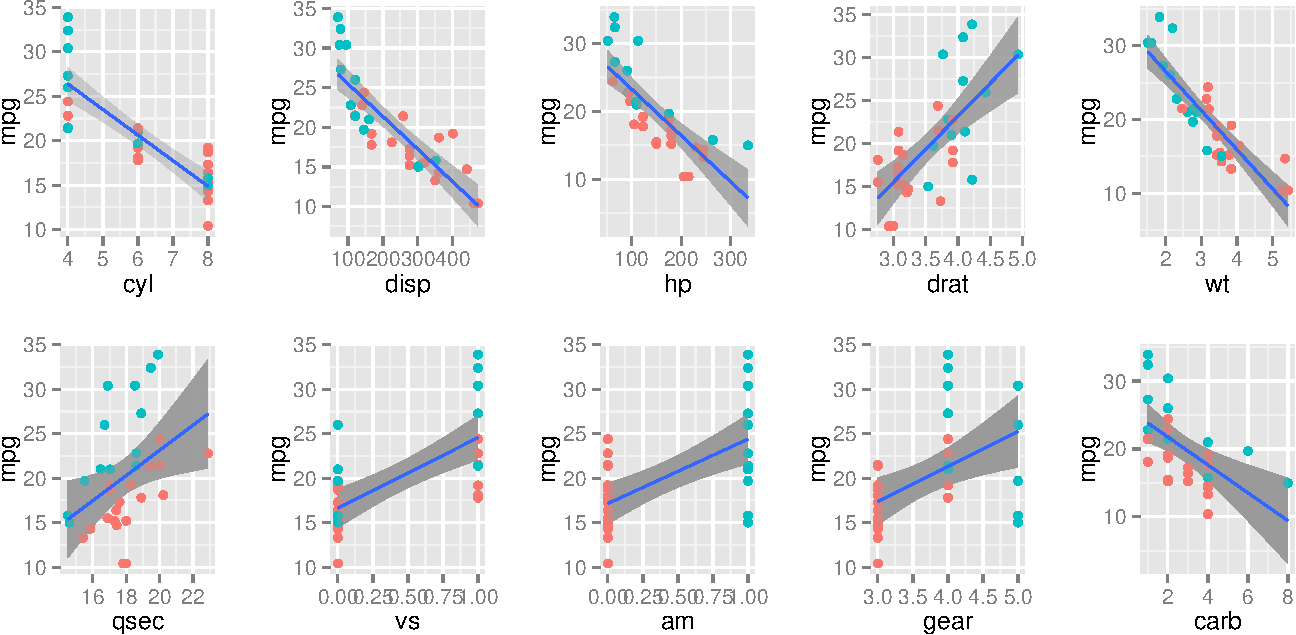
\includegraphics{coursera_regression_project_files/figure-latex/unnamed-chunk-1-1.pdf}

\subsubsection{Appendix 2}\label{appendix-2}

\begin{Shaded}
\begin{Highlighting}[]
\KeywordTok{t.test}\NormalTok{(mtcars$mpg ~}\StringTok{ }\NormalTok{mtcars$am)}
\end{Highlighting}
\end{Shaded}

\subsubsection{Appendix 3}\label{appendix-3}

\begin{Shaded}
\begin{Highlighting}[]
\NormalTok{fit_am <-}\StringTok{ }\KeywordTok{lm}\NormalTok{(mpg ~}\StringTok{ }\NormalTok{am, mtcars)}
\KeywordTok{summary}\NormalTok{(fit_am)}
\end{Highlighting}
\end{Shaded}

\subsubsection{Appendix 4}\label{appendix-4}

\begin{Shaded}
\begin{Highlighting}[]
\KeywordTok{attach}\NormalTok{(mtcars)}
\KeywordTok{cor}\NormalTok{(cyl, disp)}
\KeywordTok{t.test}\NormalTok{(disp[cyl ==}\StringTok{ }\DecValTok{4}\NormalTok{], disp[cyl ==}\StringTok{ }\DecValTok{6}\NormalTok{])}
\KeywordTok{t.test}\NormalTok{(disp[cyl ==}\StringTok{ }\DecValTok{6}\NormalTok{], disp[cyl ==}\StringTok{ }\DecValTok{8}\NormalTok{])}
\KeywordTok{summary}\NormalTok{(}\KeywordTok{lm}\NormalTok{(disp ~}\StringTok{ }\NormalTok{cyl))}
\KeywordTok{detach}\NormalTok{(mtcars)}
\end{Highlighting}
\end{Shaded}

\subsubsection{Appendix 5}\label{appendix-5}

\begin{Shaded}
\begin{Highlighting}[]
\NormalTok{fit_interaction <-}\StringTok{ }\KeywordTok{lm}\NormalTok{(mpg ~}\StringTok{ }\NormalTok{am +}\StringTok{ }\NormalTok{wt +}\StringTok{ }\NormalTok{am*wt, mtcars)}
\KeywordTok{summary}\NormalTok{(fit_interaction)$coef}
\KeywordTok{plot}\NormalTok{(mtcars$wt, mtcars$mpg, }\DataTypeTok{col =} \KeywordTok{as.factor}\NormalTok{(mtcars$am))}
\KeywordTok{abline}\NormalTok{(fit_interaction$coef[}\DecValTok{1}\NormalTok{],  fit_interaction$coef[}\DecValTok{3}\NormalTok{])}
\KeywordTok{abline}\NormalTok{(fit_interaction$coef[}\DecValTok{1}\NormalTok{] +}\StringTok{ }\NormalTok{fit_interaction$coef[}\DecValTok{2}\NormalTok{], }
       \NormalTok{fit_interaction$coef[}\DecValTok{3}\NormalTok{] +}\StringTok{ }\NormalTok{fit_interaction$coef[}\DecValTok{4}\NormalTok{], }\DataTypeTok{col =} \StringTok{"red"}\NormalTok{)}
\end{Highlighting}
\end{Shaded}

\subsubsection{Appendix 6}\label{appendix-6}

\begin{Shaded}
\begin{Highlighting}[]
\KeywordTok{summary}\NormalTok{(fit_wt)}
\KeywordTok{summary}\NormalTok{(fit_wt2)}
\end{Highlighting}
\end{Shaded}

\subsubsection{Appendix 7}\label{appendix-7}

\begin{Shaded}
\begin{Highlighting}[]
\KeywordTok{attach}\NormalTok{(mtcars)}
\KeywordTok{cor}\NormalTok{(wt, am)}
\KeywordTok{t.test}\NormalTok{(wt[am ==}\StringTok{ }\DecValTok{0}\NormalTok{], wt[am ==}\StringTok{ }\DecValTok{1}\NormalTok{])}
\KeywordTok{summary}\NormalTok{(}\KeywordTok{lm}\NormalTok{(wt ~}\StringTok{ }\NormalTok{am))}
\KeywordTok{detach}\NormalTok{(mtcars)}
\end{Highlighting}
\end{Shaded}

\subsubsection{Appendix 8}\label{appendix-8}

\begin{Shaded}
\begin{Highlighting}[]
\KeywordTok{par}\NormalTok{(}\DataTypeTok{mfrow=}\KeywordTok{c}\NormalTok{(}\DecValTok{2}\NormalTok{,}\DecValTok{2}\NormalTok{))}
\KeywordTok{plot}\NormalTok{(fit_wt2_cyl)}
\end{Highlighting}
\end{Shaded}

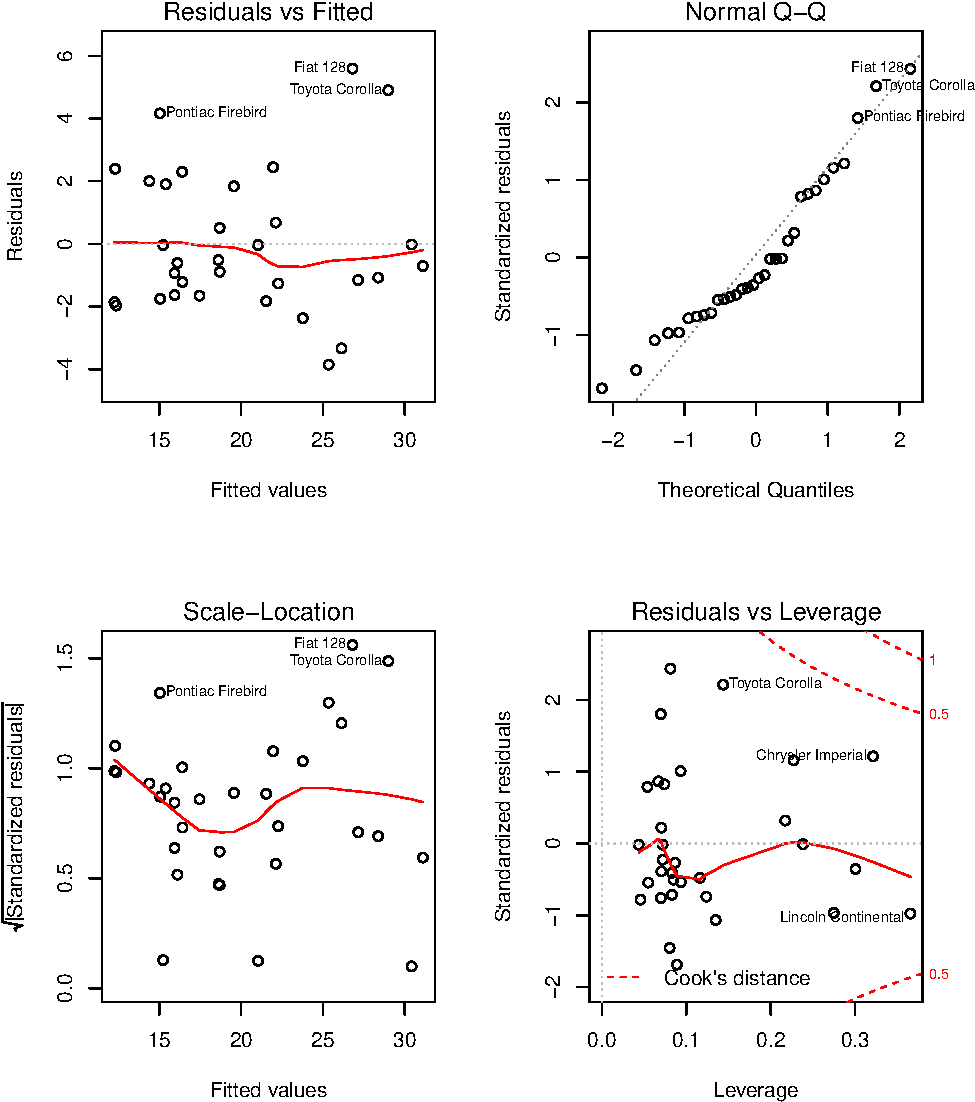
\includegraphics{coursera_regression_project_files/figure-latex/Plot residuals-1.pdf}

\end{document}
